\section{Las Vegas Grand Prix}

\subsection{Circuit Analysis}

\textbf{Circuit Name:} Las Vegas Strip Circuit (Las Vegas, United States) \\
\textbf{Length:} 6.120 km - \textbf{Laps:} 50 - \textbf{Total Distance:} 305.880 km

\begin{figure}[H]
    \centering
    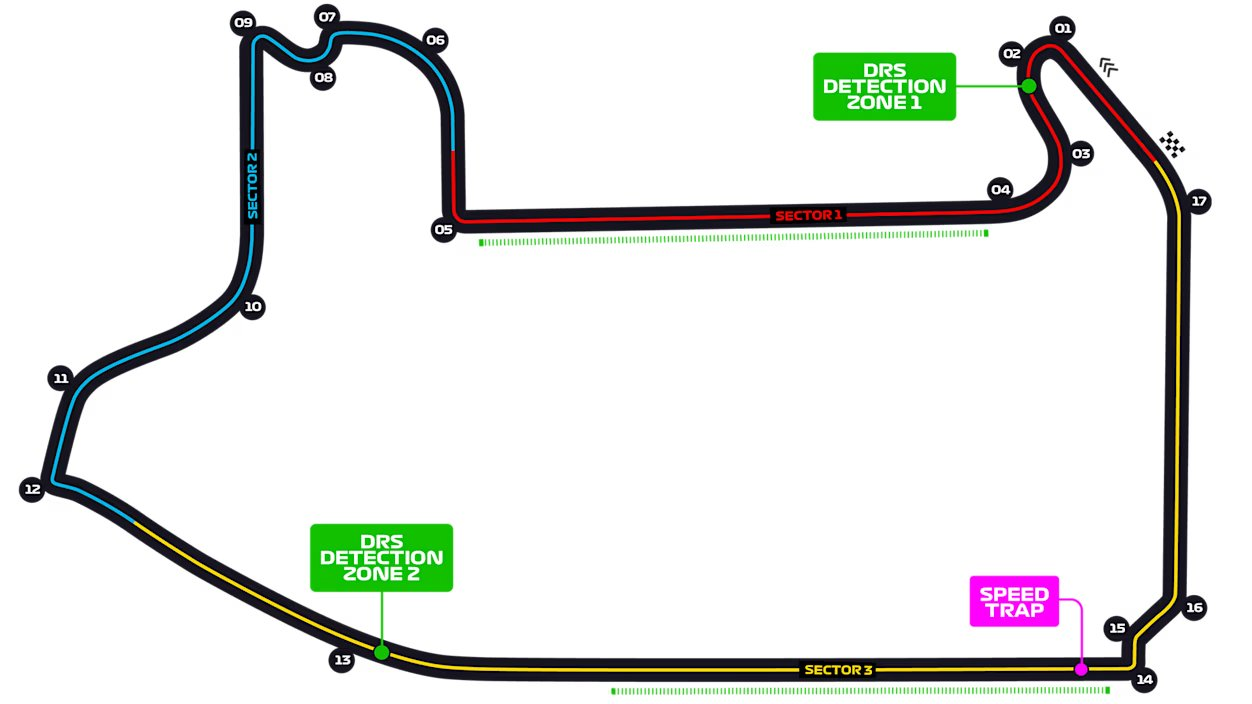
\includegraphics[width=0.75\linewidth]{images/22.Las_Vegas_Circuit.jpg}
\end{figure}

\begin{itemize}
    \item \textbf{Lap Record} : 1:32.726 (2023, Charles Leclerc - Ferrari).
    
    \item \textbf{Number of Corners \& Key Features} : 17 turns (6 right, 11 left). \\
    The layout includes a 1.9 km straight along the Strip, heavy braking zones, and long traction phases. \\
    Street circuit, wide but slippery, with bumps and cold asphalt conditions at night.
    
    \item \textbf{Braking Zones \& Traction} : Turns 1, 5, and 14 are the heaviest braking points. \\
    Grip difficult to find in cold conditions, traction at corner exits is crucial.
    
    \item \textbf{DRS \& Overtaking} : Two DRS zones: between Turns 4–5 and before Turn 14. \\
    Main overtaking opportunities into Turn 1 and Turn 14.
    
    \item \textbf{Tyre Degradation \& Strategy} : Night temperatures make tyre warm-up difficult. \\
    Surface abrasive, causing high degradation despite cool climate. \\
    Two-stop race strategies prevailed.
    
    \item \textbf{Weather \& Environment} : Cold Nevada nights (below 15°C). \\
    Low grip and tyre temperature management are defining factors. \\
    Unpredictable conditions make safety cars likely.
\end{itemize}

\textbf{Strategic Summary :} The Las Vegas Strip Circuit is defined by long straights, cold conditions, and high tyre wear. Mercedes unlocked grip where rivals failed, controlling the weekend.

\subsection{Race Analysis}

\textbf{Date:} 23 November 2024 — 22:00 local time

\begin{itemize}
    \item \textbf{Qualifying Summary} : \textbf{Pole Position:} George Russell (Mercedes) – 1:32.312 (new track record). \\
    Grid: Sainz 2nd, Gasly 3rd, Leclerc 4th. \\
    Hamilton only P10, recovered from a tough qualifying. Colapinto crashed heavily in Q2 (50g impact), started from pitlane.
    
    \item \textbf{Race Summary} : \textbf{Winner:} George Russell (Mercedes). \\
    \textbf{Podium:} 1. Russell - 2. Hamilton - 3. Sainz. \\
    Mercedes secured its 60th 1–2 finish in F1 history. \\
    Verstappen clinched his fourth World Championship despite finishing 5th, ahead of Norris (P6). \\
    \textbf{Technical issues:} Gasly (engine, lap 15), Albon (turbo, lap 25).
    
    \item \textbf{Strategies} : \\
    - Mercedes (Russell, Hamilton): two-stop (Medium–Hard–Medium), optimal under cold conditions. \\
    - Ferrari: Sainz P3, Leclerc P4 after intra-team strategy clash (Sainz ignored team orders). \\
    - Red Bull: Verstappen conservative, secured title ahead of Norris. Pérez salvaged P10. \\
    - McLaren: Norris struggled with grip, salvaged fastest lap on final lap, Piastri penalised, P7. \\
    - Haas: Hülkenberg strong P8; Magnussen just outside points. \\
    - Racing Bulls: Tsunoda P9, Lawson faded to P16. \\
    - Williams: Colapinto finished P14 after pitlane start, Albon retired.
    
    \item \textbf{Performance Trends} : \textbf{Mercedes} finally dominated: Russell untouchable, Hamilton “Driver of the Day”. \\
    \textbf{Ferrari} solid podium presence but suffered internal friction. \\
    \textbf{Red Bull} less competitive, but Verstappen achieved main target: title secured. \\
    \textbf{McLaren} off the pace on cold asphalt, limiting Norris’ comeback. \\
    \textbf{Alpine}’s high of São Paulo collapsed with Gasly’s DNF and Ocon only P17.
    
    \item \textbf{Championship Impact} : \textbf{Drivers:} Verstappen 403 pts (Champion), Norris 340, Leclerc 319. \\
    \textbf{Constructors:} McLaren 608, Ferrari 584, Red Bull 555, Mercedes 425. \\
    Constructors’ battle remains fierce: McLaren vs Ferrari vs Red Bull.
\end{itemize}

\textbf{Key Takeaway :} Mercedes conquered Las Vegas with a dominant 1–2, Russell victorious under the lights. Ferrari consistent, Red Bull focused on sealing Verstappen’s title, and McLaren underperformed but stayed in the Constructors’ lead. The championship is settled for Verstappen, but the fight between McLaren, Ferrari, and Red Bull heads until the final of the season.

\subsection{Link \& Takeaway}

\begin{itemize}
    \item Mercedes adapted best to low temperatures and tricky grip, unlocking tyre performance. 
    \item Ferrari showed pace but internal strategy disputes hindered them. 
    \item Verstappen’s cautious but efficient race secured his fourth consecutive title. 
    \item McLaren lacked consistency in cold conditions, losing ground despite fastest lap. 
    \item The Constructors’ Championship remains undecided. 
\end{itemize}
